% SPDX-License-Identifier: Apache-2.0
\section{Validation}
\label{sec:validation}

\subsection{The guards}

The derivation is not trusted. Every claim is held to a reference that
this project did not produce, or to a statement of intent made before
the database was opened.

\begin{enumerate}
  \item \emph{The VCD from the same run.} For the types it can hold,
        Vivado's own VCD is an answer key in a documented format. The
        test compares every value at every time against it.
  \item \emph{An existing parser.} That VCD is read by
        \texttt{go-vcd-parser}~\cite{govcd}, an implementation with
        its own test suite, so a bug shared between a decoder and its
        checker is avoided.
  \item \emph{The truth files.} One per case, written from the design.
  \item \emph{Independent simulators.} GHDL and nvc simulate the same
        VHDL and share no code with Vivado. Where they agree with the
        decoded database, the agreement is about the design rather
        than about one vendor's quirks.
  \item \emph{libfst on the output side.} The FST files the converter
        writes are read back with the library that defines the format
        and compared against the truth files.
\end{enumerate}

Guards~1 and~4 are blind to the same eight types the VCD omits.
Guards~3 and~5 are what cover those, which is why the FST read-back
test is not optional.

\subsection{Scale}

At the time of writing the corpus holds 1097 cases in 72 tiers. The
reader opens every one and reproduces its truth file, and the VCD
cross-check runs over every case and every design. A full test run
takes about two minutes.

\subsection{Designs from outside the project}

Small cases establish rules. Designs nobody wrote for this project
test whether the rules hold where they were not derived.

\begin{table}[t]
\caption{Designs in the test suite}
\label{tab:designs}
\centering
\begin{tabular}{llrr}
\toprule
Design & Language & Objects & Value changes \\
\midrule
\texttt{counter} (this repo) & VHDL & 14 & 2\,388 \\
\texttt{uart} (this repo) & VHDL & 59 & 16\,718 \\
SERV~\cite{serv} & Verilog & 968 & 9\,233\,899 \\
Potato~\cite{potato} & VHDL & 557 & 7\,441 \\
PicoRV32~\cite{picorv32} & Verilog & 280 & 40\,589 \\
NEORV32~\cite{neorv32} & VHDL & 5\,696 & 18\,875\,466 \\
Ibex~\cite{ibex} & SystemVerilog & 3\,287 & 73\,835 \\
\bottomrule
\end{tabular}
\end{table}

Table~\ref{tab:designs} lists them. Each taught something, or
established that there was nothing left to teach:

\begin{itemize}
  \item \emph{SERV} produced the bit offset of a Verilog port bound to
        a slice, the rule that a clocked nonblocking assignment
        records the value it already held, and the naming of a Verilog
        top elaborated with a string parameter.
  \item \emph{Potato} produced the second chunking threshold: the
        remainder of a chunked value is chunked again from 276 bytes.
        Its 32\,768 byte memories had been read as records at the
        wrong address.
  \item \emph{PicoRV32} produced nothing new, which is the expected
        result for a design in a language the corpus already covers,
        and is reported as such.
  \item \emph{Ibex}, in SystemVerilog, produced the width of an
        enumeration: it is the range the entry carries after its
        literals, and not the width of the base type, which for
        \texttt{enum logic [1:0]} is a plain \texttt{logic}. The
        reader had this right and the VCD cross check did not, so an
        enumeration inside a packed struct was compared one bit too
        narrow and every field after it moved. Tier 67 pins the rule.
  \item \emph{NEORV32} produced the rule that the chunk map belongs to
        the signal at the handle. Its DMA has an 88 byte record port
        at offset 1408 of a 1760 byte array whose initial write is
        chunked every 146 bytes, so a chunk boundary falls inside the
        port's own bytes and no single record covers it. The reader
        refused the file on 39 of its 5696 objects. The correction is
        four lines; finding it took a design of that size.
\end{itemize}

\begin{figure*}[t]
  \centering
  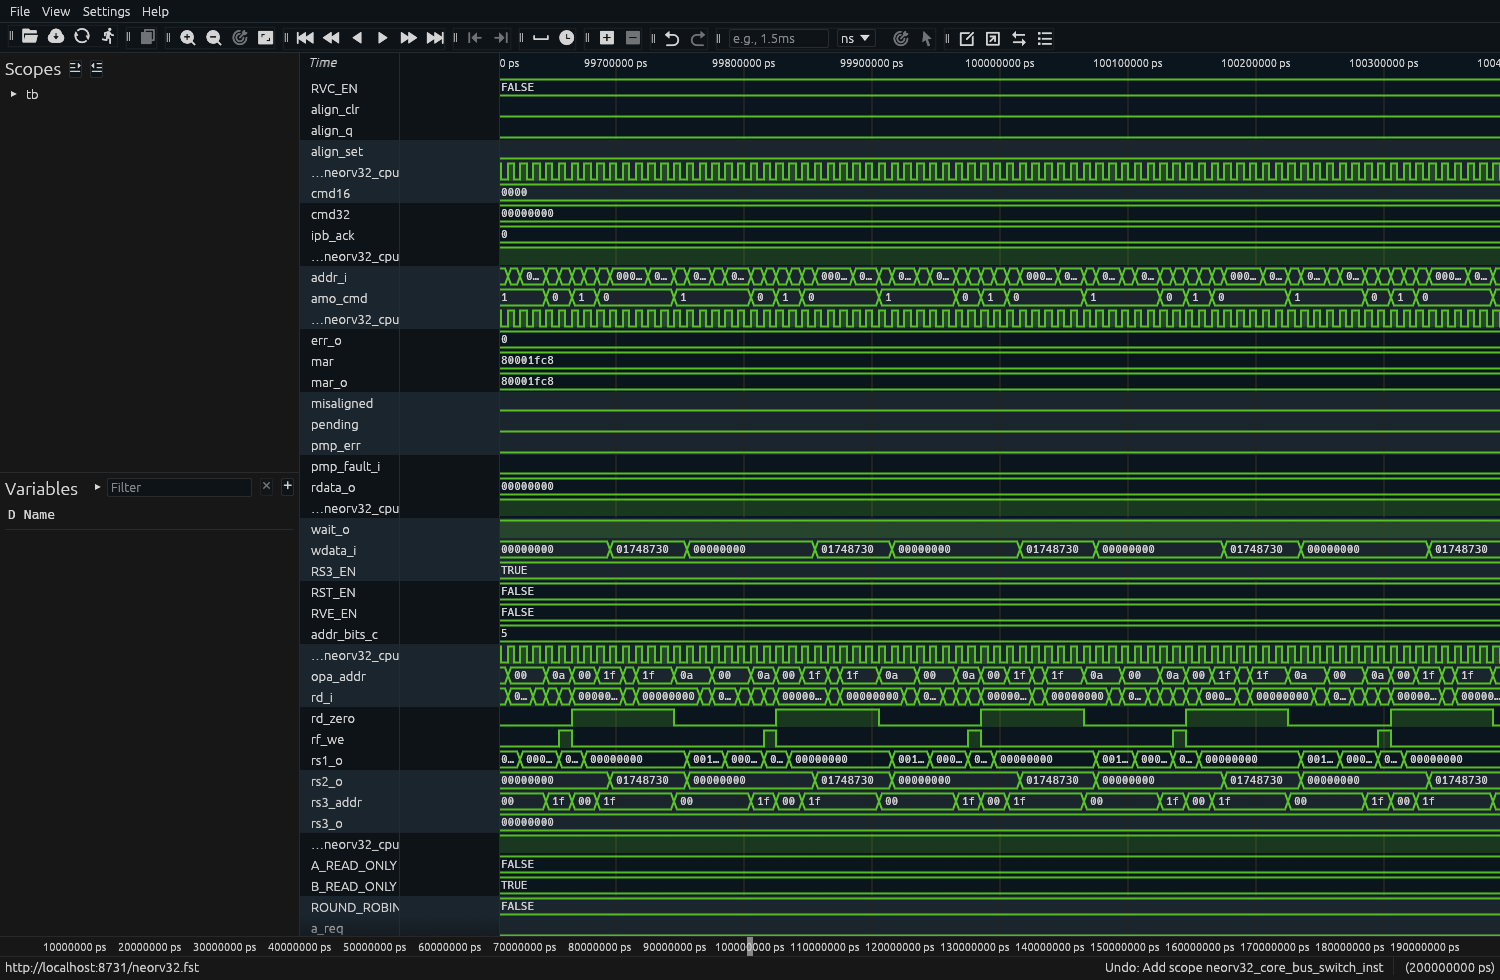
\includegraphics[width=\textwidth]{figures/neorv32-soc-surfer.png}
  \caption{The largest design in the suite after conversion: signals
  from four modules of one NEORV32 core at once, the instruction
  frontend, the load and store unit, the register file and the bus
  switch between them. The database holds 5696 objects in 4832 scopes;
  the rows that read \texttt{TRUE} and \texttt{FALSE} are VHDL
  generics, and the rows that read \texttt{80001fc8} are integers and
  vectors, none of which Vivado's VCD of the same run declares.}
  \label{fig:soc}
\end{figure*}

Fig.~\ref{fig:soc} shows that design after conversion, with signals
from four of its modules on one screen. A design of that size is also
the only kind that exercises the parts of the format a small case
never reaches, which is what the two defects above have in common.

\subsection{A defect found in the checker}

NEORV32 also exposed a limitation in the VCD parser used as guard~2. A
VCD identifier code may be any printable ASCII, and a design with
enough variables receives codes such as \texttt{\#0}, which the
parser's lexer read as a timestamp, and \texttt{R0}, which it read as
a real. The fix, a lexer state in which the word after a value is the
identifier code whatever it looks like, was contributed upstream.
